\documentclass[12pt]{jarticle}
\usepackage[dvipdfmx]{graphicx}
\usepackage[dvipdfmx]{color}
\usepackage{here}
\title{原子核の変形と中性子ドリップラインに対するクーロン相互作用の効果}
\author{萩原健太}
\date{2023年1月21日}
\begin{document}

\begin{center}
    {\Large
        原子核の変形と中性子ドリップラインに対するクーロン相互作用の効果
    }
\end{center}

\begin{flushright}
  \\201910867 萩原健太\\
  指導教員:中務孝 日野原伸生
\end{flushright}

\section{結果}
陽子数$Z=2$から$Z=120$の偶偶核の計算を実行し、陽子、中性子のchemical potentialがともに負の原子核の変形度を (図\ref{fig:SLY4_ON})にプロットした。
変形度は軸対象の変形を示しており、絶対値で表示している。
(図\ref{fig:SLY4_OFF})にはクーロン相互作用を外した場合の計算結果を示す。
これらの結果よりクーロン相互作用の有無によって核図表全体に渡って変形度が増加していること、および質量数の大きな領域では中性子ドリップラインが拡大していることが確認できる。
\begin{figure}[ht]
    \centering
    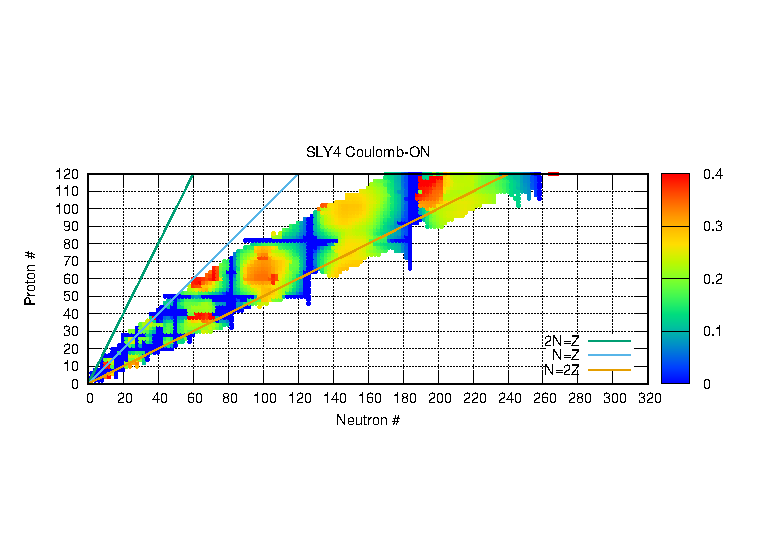
\includegraphics{SLY4_ON.eps}
    \setlength\floatsep{0pt}
    \setlength\intextsep{0pt} 
    \setlength\textfloatsep{0pt}
    \caption{SLY4 Coulomb-ON}
    label{fig:SLY4_ON}
\end{figure}
\begin{figure}[ht]
    \centering
    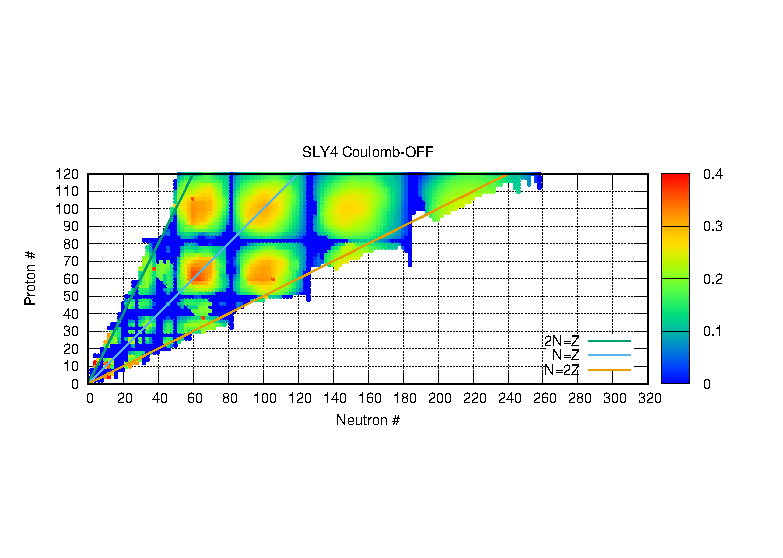
\includegraphics{SLY4_OFF.eps}
    \setlength\floatsep{0pt}
    \caption{SLY4 Coulomb-OFF}
    label{fig:SLY4_OFF}
\end{figure}

またクーロン相互作用と原子核の半径にも相関があることが明らかになった。
(図/ref{fig:SLY4_Z=50_radius_and_beta})~ (図/ref{fig:SLY4_Z=50_radius_and_beta})には$Z=50$の変形度$\beta$と半径を、中性子数の関数として表示した。
これらの図から変形がない領域でも半径が増加し、変形の有無に依らず、クーロン相互作用によって原子核の半径は増加することが確認できる。

\subsection{変形度に関する考察}
続いてクーロン相互作用の有無で、原子核の基底状態における変形度がどの程度変化するのか調べた。


\end{document}